\documentclass{ximera}

%\usepackage{todonotes}

\newcommand{\todo}{}

\usepackage{tkz-euclide}
\tikzset{>=stealth} %% cool arrow head
\tikzset{shorten <>/.style={ shorten >=#1, shorten <=#1 } } %% allows shorter vectors

\usepackage{tkz-tab}  %% sign charts
\usetikzlibrary{decorations.pathreplacing} 

\usetikzlibrary{backgrounds} %% for boxes around graphs
\usetikzlibrary{shapes,positioning}  %% Clouds and stars
\usetikzlibrary{matrix} %% for matrix
\usepgfplotslibrary{polar} %% for polar plots
\usetkzobj{all}
\usepackage[makeroom]{cancel} %% for strike outs
%\usepackage{mathtools} %% for pretty underbrace % Breaks Ximera
\usepackage{multicol}

\usepackage{polynom}



\usepackage[many]{tcolorbox}  %% for titled boxes
\newtcolorbox{xbox}[1]{%
    tikznode boxed title,
    enhanced,
    arc=0mm,
    interior style={white},
    attach boxed title to top center= {yshift=-\tcboxedtitleheight/2},
    fonttitle=\bfseries,
    colbacktitle=white,coltitle=black,
    boxed title style={size=normal,colframe=white,boxrule=0pt},
    title={#1}}


\usepackage{array}
\setlength{\extrarowheight}{+.1cm}   
\newdimen\digitwidth
\settowidth\digitwidth{9}
\def\divrule#1#2{
\noalign{\moveright#1\digitwidth
\vbox{\hrule width#2\digitwidth}}}





\newcommand{\RR}{\mathbb R}
\newcommand{\R}{\mathbb R}
\newcommand{\N}{\mathbb N}
\newcommand{\Z}{\mathbb Z}

%\renewcommand{\d}{\,d\!}
\renewcommand{\d}{\mathop{}\!d}
\newcommand{\dd}[2][]{\frac{\d #1}{\d #2}}
\newcommand{\pp}[2][]{\frac{\partial #1}{\partial #2}}
\renewcommand{\l}{\ell}
\newcommand{\ddx}{\frac{d}{\d x}}
\newcommand{\ddt}{\frac{d}{\d t}}

\newcommand{\zeroOverZero}{\ensuremath{\boldsymbol{\tfrac{0}{0}}}}
\newcommand{\inftyOverInfty}{\ensuremath{\boldsymbol{\tfrac{\infty}{\infty}}}}
\newcommand{\zeroOverInfty}{\ensuremath{\boldsymbol{\tfrac{0}{\infty}}}}
\newcommand{\zeroTimesInfty}{\ensuremath{\small\boldsymbol{0\cdot \infty}}}
\newcommand{\inftyMinusInfty}{\ensuremath{\small\boldsymbol{\infty - \infty}}}
\newcommand{\oneToInfty}{\ensuremath{\boldsymbol{1^\infty}}}
\newcommand{\zeroToZero}{\ensuremath{\boldsymbol{0^0}}}
\newcommand{\inftyToZero}{\ensuremath{\boldsymbol{\infty^0}}}



\newcommand{\numOverZero}{\ensuremath{\boldsymbol{\tfrac{\#}{0}}}}
\newcommand{\dfn}{\textbf}
%\newcommand{\unit}{\,\mathrm}
\newcommand{\unit}{\mathop{}\!\mathrm}
\newcommand{\eval}[1]{\bigg[ #1 \bigg]}
\newcommand{\seq}[1]{\left( #1 \right)}
\renewcommand{\epsilon}{\varepsilon}
\renewcommand{\iff}{\Leftrightarrow}

\DeclareMathOperator{\arccot}{arccot}
\DeclareMathOperator{\arcsec}{arcsec}
\DeclareMathOperator{\arccsc}{arccsc}
\DeclareMathOperator{\si}{Si}
\DeclareMathOperator{\proj}{proj}
\DeclareMathOperator{\scal}{scal}


\newcommand{\tightoverset}[2]{% for arrow vec
  \mathop{#2}\limits^{\vbox to -.5ex{\kern-0.75ex\hbox{$#1$}\vss}}}
\newcommand{\arrowvec}[1]{\tightoverset{\scriptstyle\rightharpoonup}{#1}}
\renewcommand{\vec}{\mathbf}
\newcommand{\veci}{\vec{i}}
\newcommand{\vecj}{\vec{j}}
\newcommand{\veck}{\vec{k}}
\newcommand{\vecl}{\boldsymbol{\l}}

\newcommand{\dotp}{\bullet}
\newcommand{\cross}{\boldsymbol\times}
\newcommand{\grad}{\boldsymbol\nabla}
\newcommand{\divergence}{\grad\dotp}
\newcommand{\curl}{\grad\cross}
%\DeclareMathOperator{\divergence}{divergence}
%\DeclareMathOperator{\curl}[1]{\grad\cross #1}


\colorlet{textColor}{black} 
\colorlet{background}{white}
\colorlet{penColor}{blue!50!black} % Color of a curve in a plot
\colorlet{penColor2}{red!50!black}% Color of a curve in a plot
\colorlet{penColor3}{red!50!blue} % Color of a curve in a plot
\colorlet{penColor4}{green!50!black} % Color of a curve in a plot
\colorlet{penColor5}{orange!80!black} % Color of a curve in a plot
\colorlet{fill1}{penColor!20} % Color of fill in a plot
\colorlet{fill2}{penColor2!20} % Color of fill in a plot
\colorlet{fillp}{fill1} % Color of positive area
\colorlet{filln}{penColor2!20} % Color of negative area
\colorlet{fill3}{penColor3!20} % Fill
\colorlet{fill4}{penColor4!20} % Fill
\colorlet{fill5}{penColor5!20} % Fill
\colorlet{gridColor}{gray!50} % Color of grid in a plot

\newcommand{\surfaceColor}{violet}
\newcommand{\surfaceColorTwo}{redyellow}
\newcommand{\sliceColor}{greenyellow}




\pgfmathdeclarefunction{gauss}{2}{% gives gaussian
  \pgfmathparse{1/(#2*sqrt(2*pi))*exp(-((x-#1)^2)/(2*#2^2))}%
}


%%%%%%%%%%%%%
%% Vectors
%%%%%%%%%%%%%

%% Simple horiz vectors
\renewcommand{\vector}[1]{\left\langle #1\right\rangle}


%% %% Complex Horiz Vectors with angle brackets
%% \makeatletter
%% \renewcommand{\vector}[2][ , ]{\left\langle%
%%   \def\nextitem{\def\nextitem{#1}}%
%%   \@for \el:=#2\do{\nextitem\el}\right\rangle%
%% }
%% \makeatother

%% %% Vertical Vectors
%% \def\vector#1{\begin{bmatrix}\vecListA#1,,\end{bmatrix}}
%% \def\vecListA#1,{\if,#1,\else #1\cr \expandafter \vecListA \fi}

%%%%%%%%%%%%%
%% End of vectors
%%%%%%%%%%%%%

%\newcommand{\fullwidth}{}
%\newcommand{\normalwidth}{}



%% makes a snazzy t-chart for evaluating functions
%\newenvironment{tchart}{\rowcolors{2}{}{background!90!textColor}\array}{\endarray}

%%This is to help with formatting on future title pages.
\newenvironment{sectionOutcomes}{}{} 



%% Flowchart stuff
%\tikzstyle{startstop} = [rectangle, rounded corners, minimum width=3cm, minimum height=1cm,text centered, draw=black]
%\tikzstyle{question} = [rectangle, minimum width=3cm, minimum height=1cm, text centered, draw=black]
%\tikzstyle{decision} = [trapezium, trapezium left angle=70, trapezium right angle=110, minimum width=3cm, minimum height=1cm, text centered, draw=black]
%\tikzstyle{question} = [rectangle, rounded corners, minimum width=3cm, minimum height=1cm,text centered, draw=black]
%\tikzstyle{process} = [rectangle, minimum width=3cm, minimum height=1cm, text centered, draw=black]
%\tikzstyle{decision} = [trapezium, trapezium left angle=70, trapezium right angle=110, minimum width=3cm, minimum height=1cm, text centered, draw=black]


\outcome{Use the first derivative to determine whether a function is increasing or decreasing.}

\author{Nela Lakos \and Kyle Parsons}

\begin{document}
\begin{exercise}

An object begins moving along a vertical line at time $t=0$s and stops at time $t=6$s.  Its height above the ground at time $t$ is given by $h(t)$ depicted in the graph below, where $h$ is measured in meters.

\begin{image}
  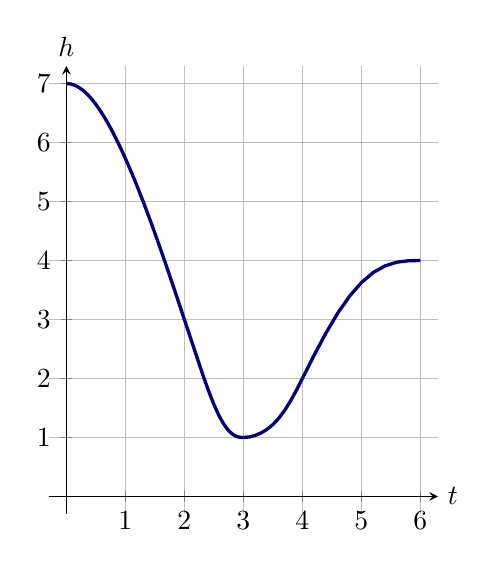
\begin{tikzpicture}
    \begin{axis}[
        xmin=-0.3,xmax=6.3,ymin=-0.3,ymax=7.3,
        clip=true,
        unit vector ratio*=1 1 1,
        axis lines=center,
        grid = major,
        ytick={0,1,...,7},
    xtick={0,1,...,6},
        xlabel=$t$, ylabel=$h$,
        every axis y label/.style={at=(current axis.above origin),anchor=south},
        every axis x label/.style={at=(current axis.right of origin),anchor=west},
      ]
      %\addplot[very thick,penColor,domain=0:3,samples=50] plot{6/(1+e^(3.4*(x-1.5)))+1};
      %\addplot[very thick,penColor,domain=3:6,samples=50] plot{3/(1+e^(3*(-x+4.5)))+1};
      \addplot[very thick,penColor,domain=0:2,samples=50] plot{-x^7/96 + 3*x^6/32 - 5*x^5/16 + 11*x^4/24 - 3*x^2/2 + 7};
      \addplot[very thick,penColor,domain=2:3,samples=50] plot{-2*x^5 + 24*x^4 - 113*x^3 + 262*x^2 - 303*x + 145};
      %\addplot[very thick,penColor,domain=3:4,samples=50] plot{-1*x^5 + 17*x^4 - 115*x^3 + 338*x^2 - 654*x + 442};
      %\addplot[very thick,penColor,domain=3:4,samples=50] plot{442 - x^5 + 17*x^4 - 654*x + 338*x^2 - 115*x^3};
      \draw[very thick,penColor,smooth] (axis cs:3,1)
      									-- (axis cs:3.1,1.00919)
										-- (axis cs:3.2,1.03488)
									 	-- (axis cs:3.3,1.07677)
										-- (axis cs:3.4,1.13696)
										-- (axis cs:3.5,1.21875)
										-- (axis cs:3.6,1.32544)
										-- (axis cs:3.7,1.45913)
										-- (axis cs:3.8,1.61952)
										-- (axis cs:3.9,1.80271)
      									-- (axis cs:4,2);
      \draw[very thick,penColor,smooth] (axis cs:4,2)
      									-- (axis cs:4.2,2.3962)
										-- (axis cs:4.4,2.7712)
										-- (axis cs:4.6,3.1082)
										-- (axis cs:4.8,3.3952)
										-- (axis cs:5,29/8)
										-- (axis cs:5.2,3.7952)
										-- (axis cs:5.4,3.9082)
										-- (axis cs:5.6,3.9712)
										-- (axis cs:5.8,3.9962)
										-- (axis cs:6,4);
      %\addplot[very thick,penColor,domain=4:6,samples=5,smooth] plot{x^4/8 - 5*x^3/2 + 18*x^2 - 54*x + 58};
      \end{axis}`
  \end{tikzpicture}
\end{image}

The average velocity of the object on the interval $\left[0,6\right]$ is
\[
v_{\text{av}} = \answer{-\frac{1}{2}}\text{m/s}.
\]

Choose the best description of the shape of the graph on the time interval $\left(0,1\right)$.
\begin{multipleChoice}
\choice{Increasing and concave up}
\choice{Increasing and concave down}
\choice{Decreasing and concave up}
\choice[correct]{Decreasing and concave down}
\end{multipleChoice}

The object is closest to the ground at 
\[
t=\answer{3}\text{s}.
\]

The velocity when the object is closest to the ground is 
\[
v=\answer{0}\text{m/s}.
\]

At which time is the velocity greatest?
\begin{multipleChoice}
\choice{0s}
\choice{2s}
\choice{3s}
\choice[correct]{4s}
\choice{6s}
\end{multipleChoice}

Estimated as an integer, the maximum velocity is
\[
v=\answer{2}\text{m/s}.
\]

Let $v(t)$ be the velocity of the object at time $t$.  Chose the greatest value amongst the following choices.
\begin{multipleChoice}
\choice[correct]{$v(4.5)$}
\choice{$v(4.6)$}
\choice{$v(4.7)$}
\choice{$v(4.8)$}
\end{multipleChoice}

The time interval on which the velocity is increasing is
\[
\left(\answer{2},\answer{4}\right).
\]

At which of the following times is speed greatest?
\begin{multipleChoice}
\choice{1s}
\choice[correct]{2s}
\choice{3s}
\choice{4s}
\end{multipleChoice}

\end{exercise}
\end{document}